\subsection{TOPOLOGIES ON GROUPS OF HOMEOMORPHISMS}

PROPOSITION 10. Let X be a uniform space and let H be an equicontinuous set of homeomorphisms of X onto itself. If H and \(H^{-1}\) are endowed with the topology of pointwise convergence in X, then the mapping \(u \rightarrow u^{-1}\) of \(H^{-1}\) onto H is continuous.

It is enough to show that, for each \(x_0 \in \mathbf{X}\) , the mapping \(u \to u^{-1}(x_0)\) of \(\mathbf{H}^{-1}\) into \(\mathbf{X}\) is continuous at every point \(u_0 \in \mathbf{H}^{-1}\) . Let \(\mathbf{V}\) be a symmetric entourage of \(\mathbf{X}\) , and let \(y_0 = u_0^{-1}(x_0)\) . By hypothesis there is a symmetric entourage \(\mathbf{U}\) of \(\mathbf{X}\) such that the relation \((x, x_0) \in \mathbf{U}\) implies \((u^{-1}(x), u^{-1}(x_0)) \in \mathbf{V}\) for all \(u \in \mathbf{H}^{-1}\) . Take an element \(u \in \mathbf{H}^{-1}\) which is \(W(\{y_0\}, \mathbf{U})\) -close to \(u_0\) ; then we have \((u(y_0), u_0(y_0)) \in \mathbf{U}\) , i.e.~\((u(y_0), x_0) \in \mathbf{U}\) . It follows that \((y_0, u^{-1}(x_0)) \in \mathbf{V}\) , i.e.~\((u_0^{-1}(x_0), u^{-1}(x_0)) \in \mathbf{V}\) ; this completes the proof.

COROLLARY. Let X be a uniform space and let H be an equicontinuous group of homeomorphisms of X onto itself. Then the topology of pointwise convergence in X is compatible with the group structure of H.

This is a consequence of Proposition 10, together with § 2, no. 1, Proposition 1, Corollary 5.

PROPOSITION II. Let X be a compact space and let \(\Gamma\) be the group of all homeomorphisms of X onto itself. Then the topology of uniform convergence in X is compatible with the group structure of \(\Gamma\) .

We know already (no. 4, Proposition 9) that the mapping \((u, v) \to v \circ u\) of \(\Gamma \times \Gamma\) into \(\Gamma\) is continuous with respect to this topology; thus we have to show that \(u \to u^{-1}\) is continuous at every point \(u_0\) of \(\Gamma\) . Since \(u_0^{-1}\) is uniformly continuous on \(\mathbf{X}\) , given any symmetric entourage \(\mathbf{V}\) of \(\mathbf{X}\) there exists an entourage \(\mathbf{W}\) of \(\mathbf{X}\) such that the relation \((x, x') \in \mathbf{W}\) implies \((u_0^{-1}(x), u_0^{-1}(x')) \in \mathbf{V}\) . Hence, if \(u \in \Gamma\) is such that \((u_0(x), u(x)) \in \mathbf{W}\) for all \(x \in \mathbf{X}\) , it follows that \((x, u_0^{-1}(u(x))) \in \mathbf{V}\) for all \(x \in \mathbf{X}\) , and therefore (as \(u\) is bijective) \((u^{-1}(x), u_0^{-1}(x)) \in \mathbf{V}\) for all \(x \in \mathbf{X}\) . This completes the proof.

\pandocbounded{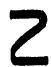
\includegraphics[keepaspectratio]{images/part002_d26bd6ea.jpg}}

Now let X be a locally compact space and let \(\Gamma\) be the group of all homeomorphisms of X onto itself. The topology of compact convergence in X is not necessarily compatible with the group structure of \(\Gamma\) (Exercise 17). Let \(X'\) denote the compact space obtained by adjoining a point at infinity \(\omega\) to X. Every homeomorphism u of X onto itself extends uniquely to a homeomorphism \(u'\) of \(X'\) onto itself such that \(u'(\omega) = \omega\) (Chapter I, § 10, no. 3, Corollary to Proposition 7), so that \(\Gamma\) can be identified with the subgroup of the group \(\Gamma'\) of all homeomorphisms of \(X'\) onto itself, consisting of all homeomorphisms which leave \(\omega\) fixed. The topology induced on \(\Gamma\) by that of \(C_u(X'; X')\) is therefore compatible with the group structure of \(\Gamma\) (Proposition 11), and \(\Gamma\) is closed in \(\Gamma'\) {[}with respect to the topology induced by that of \(\mathcal{C}_u(\mathbf{X}';\mathbf{X}')\) {]} because it is defined by the equation \(u(\omega)=\omega\) ( \(\S\) 1, no. 2, Remark 6). We denote by \(\mathcal{C}_{\beta}\) the group topology thus defined on \(\Gamma\) ; it is finer than the topology of compact convergence and can also (by virtue of \(\S\) 1, no. 6, Proposition 6) be defined as the topology of uniform convergence on \(\mathbf{X}\) , when \(\mathbf{X}\) is endowed with the uniformity induced by the unique uniformity of \(\mathbf{X}'\) .

The topology \(\mathcal{C}_{\beta}\) can be characterized as follows:

PROPOSITION 12. On the group \(\Gamma\) of all homeomorphisms of a locally compact space \(\mathbf{X}\) , the topology \(\mathcal{C}_{\beta}\) is the coarsest for which the mappings \(u \to u\) and \(u \to u^{-1}\) of \(\Gamma\) into \(\mathcal{C}_c(\mathbf{X}; \mathbf{X})\) are continuous.

Let us denote the latter topology for the moment by \(\mathcal{C}'\) . Since \(u \to u^{-1}\) is continuous with respect to \(\mathcal{C}_{\beta}\) and since \(\mathcal{C}_{\beta}\) is finer than the topology of compact convergence, it is clear that \(\mathcal{C}_{\beta}\) is finer than \(\mathcal{C}'\) . To prove the converse, endow \(\mathbf{X}'\) with its unique uniformity; let \(u_0 \in \Gamma\) and let \(\mathbf{V}\) be an entourage of \(\mathbf{X}'\) ; then we have to prove that there is a compact subset \(\mathbf{K}\) of \(\mathbf{X}\) and a symmetric entourage \(\mathbf{W}\) of \(\mathbf{X}'\) such that the relations

\[
u \in \Gamma , (u _ {0} (x), u (x)) \in \mathrm{W} \text {   and   } (u _ {0} ^ {- 1} (x), u ^ {- 1} (x)) \in \mathrm{W} \text {   for   all   } x \in \mathrm{K}
\]

imply

\[
(u _ {0} (x), u (x)) \in \mathbf {V} \text {   for   all   } x \in \mathbf {X}.
\]

Let \(V_1\) be a symmetric open entourage of \(X'\) such that \(\dot{V}_1 \subset V\) ; then \(K_1 = X' - V_1(\omega)\) is a compact subset of \(X\) . Choose a symmetric open entourage \(W\) of \(X'\) such that \(W \subset V\) and \(W(\omega) \cap W(u_0^{-1}(K_1)) = \emptyset\) ; this is possible by Proposition 4 of Chapter II, § 4, no. 3. Let \(K_2 = X' - W(\omega)\) , which is a compact subset of \(X\) . We shall see that \(W\) and the compact set \(K = K_1 \cup K_2\) do what is required. Since \(W \subset V\) , it is enough to show that the relation

\[
\left(u _ {0} ^ {- 1} (x), u ^ {- 1} (x)\right) \in \mathrm{W} \quad \text { for   all } \quad x \in \mathrm{K} _ {1} \quad (u \in \Gamma)
\]

implies that

\[
(u (y), \omega) \in \mathrm{V} _ {1} \quad \text { for   all } \quad y \in \mathrm{W} (\omega);
\]

for we shall then also have \((u_0(y),\omega)\in \mathbf{V}_1\) and thence

\[
(u _ {0} (y), u (y)) \in \mathring {\mathrm{V}} _ {1} ^ {2} \subset \mathrm{V}
\]

for all \(y \in W(\omega) = X' - K_2\) . Now if we had \(y \in W(\omega)\) and

\[
u (y) \in \mathrm{X} ^ {\prime} - \mathrm{V} _ {1} (\omega) = \mathrm{K} _ {1},
\]

it would follow that \(y \in u^{-1}(\mathbf{K}_1) \subset W(u_0^{-1}(\mathbf{K}_1))\) , contrary to the choice of \(W\) ; the proof is therefore complete.

In general the group \(\Gamma\) , endowed with \(\mathfrak{G}_{\beta}\) , is not locally compact; but we have the following criterion:

THEOREM 4. Let G be a subgroup of the group \(\Gamma\) of all homeomorphisms of a locally compact space X. Suppose that, in the space \(\mathcal{C}_{\mathfrak{c}}(\mathbf{X};\mathbf{X})\) , there is a neighbourhood V of the identity mapping \(e\) such that \(\mathbf{V}\cap \mathbf{G} = \mathbf{H}\) is symmetric in G and relatively compact in \(\mathcal{C}_{\mathfrak{c}}(\mathbf{X};\mathbf{X})\) . Then the closure \(\overline{\mathbf{G}}\) of G in \(\Gamma\) with respect to the topology \(\mathcal{T}_{\beta}\) is a locally compact group with respect to the topology induced by \(\mathcal{T}_{\beta}\) ; this topology induced on \(\overline{\mathbf{G}}\) is the same as the topology of compact convergence, and the closure \(\overline{\mathbf{H}}\) of H in \(\mathcal{C}_{\mathfrak{c}}(\mathbf{X};\mathbf{X})\) is a neighbourhood of \(e\) in \(\overline{\mathbf{G}}\) with respect to this topology.

Let us show first that \(\overline{\mathbf{H}}\) is contained in \(\Gamma\) and that the topology induced on \(\overline{\mathbf{H}}\) by \(\mathfrak{C}_{\beta}\) is the same as the topology of compact convergence. Let \(u_0 \in \overline{\mathbf{H}}\) ; \(u_0\) is therefore the limit, in \(\mathcal{C}_c(\mathbf{X}; \mathbf{X})\) , of an ultrafilter \(\Phi\) on \(\mathbf{H}\) . Since \(\Phi^{-1}\) (the image of \(\Phi\) under \(u \to u^{-1}\) ) is an ultrafilter base on \(\mathbf{H} \subset \overline{\mathbf{H}}\) , it converges in the compact subspace \(\overline{\mathbf{H}}\) of \(\mathcal{C}_c(\mathbf{X}; \mathbf{X})\) to an element \(v_0\) . The mapping \((u, v) \to uv\) converges to \(u_0 v_0\) with respect to \(\Phi \times \Phi^{-1}\) (no. 4, Proposition 9); a fortiori, \(u \to uu^{-1} = e\) converges to \(u_0 v_0\) with respect to \(\Phi\) , hence \(u_0 v_0 = e\) since \(\mathcal{C}_c(\mathbf{X}; \mathbf{X})\) is Hausdorff. Similarly \(v_0 u_0 = e\) ; hence \(u_0\) is a homeomorphism of \(\mathbf{X}\) , i.e., \(u_0 \in \Gamma\) . Thus \(\overline{\mathbf{H}}\) is contained in \(\Gamma\) . Moreover, this argument shows that \(\overline{\mathbf{H}}^{-1} = \overline{\mathbf{H}}\) and that, for every ultrafilter \(\Phi\) on \(\overline{\mathbf{H}}\) which converges to \(u_0\) , \(\Phi^{-1}\) converges in \(\mathcal{C}_c(\mathbf{X}; \mathbf{X})\) to \(u_0^{-1}\) ; hence the mapping \(u \to u^{-1}\) of \(\overline{\mathbf{H}}\) into \(\mathcal{C}_c(\mathbf{X}; \mathbf{X})\) is continuous when \(\overline{\mathbf{H}}\) carries the topology of compact convergence (Chapter I, § 7, no. 4, Proposition 9, Corollary 1). Proposition 12 then shows that, on \(\overline{\mathbf{H}}\) , the topology of compact convergence is the same as the topology induced by \(\mathfrak{C}_{\beta}\) .

Furthermore, since the topology \(\mathcal{C}_{\beta}\) on \(\Gamma\) is finer than the topology of compact convergence, \(\overline{\mathbf{H}}\) is also the closure of \(\mathbf{H}\) with respect to \(\mathcal{C}_{\beta}\) . But \(\mathbf{H}\) is a neighbourhood of \(e\) in \(\mathbf{G}\) with respect to the topology of compact convergence, and a fortiori with respect to the topology induced by \(\mathcal{C}_{\beta}\) ; it follows (Chapter I, § 3, no. 1, Proposition 2) that \(\overline{\mathbf{H}}\) is a neighbourhood of \(e\) in \(\overline{\mathbf{G}}\) with respect to the topology induced by \(\mathcal{C}_{\beta}\) , and hence \(\overline{\mathbf{G}}\) is locally compact in this topology. If \(\mathbf{W}\) is the interior of \(\mathbf{V}\) with respect to the topology of compact convergence, then \(\mathbf{W} \cap \Gamma\) is open in \(\mathcal{C}_{\beta}\) , hence \(\mathbf{W} \cap \overline{\mathbf{G}}\) is contained in the closure of \(\mathbf{H} = \mathbf{V} \cap \mathbf{G}\) with respect to \(\mathcal{C}_{\beta}\) (Chapter I, § 1, no. 6, Proposition 5); this shows that \(\overline{\mathbf{H}}\) is also a neighbourhood of \(e\) in \(\overline{\mathbf{G}}\) with respect to the topology of compact convergence. Finally, for each \(u_{0} \in \Gamma\) , the bijections \(v \to u_{0} \circ v\) and \(v \to u_{0}^{-1} \circ v\) of \(\mathcal{C}_{c}(\mathbf{X}; \mathbf{X})\) onto itself are continuous (no. 4, Proposition 9), and hence, if \(u_{0} \in \overline{G}\) , \(u_{0}\overline{H}\) is a neighbourhood of \(u_{0}\) in \(\overline{G}\) with respect to the topology of compact convergence. This completes the proof.

COROLLARY. Let G be a group of homeomorphisms of a locally compact space X. If the closure \(\overline{G}\) of G in \(\mathcal{C}_{c}(X; X)\) is compact, then \(\overline{G}\) is a group of homeomorphisms of X, and the topology of compact convergence is compatible with the group structure of \(\overline{G}\) , which is therefore a compact topological group.

\pandocbounded{
\includegraphics[keepaspectratio]{images/part002_e2b18e11.jpg}}

A group of homeomorphisms of a locally compact space X which is locally compact but not compact with respect to the topology of compact convergence is locally closed in \(\mathcal{C}_{c}(\mathbf{X};\mathbf{X})\) by virtue of Chapter I, § 9, no. 7, Proposition 12, but is not necessarily closed.

For example, in the ring \(\mathcal{L}(\mathbf{R}^{n})\) of endomorphisms of \(\mathbf{R}^{n}\) , identified with the ring \(\mathbf{M}_{n}(\mathbf{R})\) of square \(n \times n\) matrices over \(\mathbf{R}\) and endowed with the topology of compact convergence, the group \(\mathbf{GL}(n, \mathbf{R})\) , identified with the group of non-singular matrices, is locally compact but dense (Chapter VI, § 1, no. 6, Proposition 6).

